\documentclass[a4paper]{article}
\usepackage{mathtools}
\usepackage{pdfpages}
\usepackage{graphicx}
\usepackage{geometry}

\geometry{
  a4paper,
  total={170mm,257mm},
  left=20mm,
  top=20mm,
}

\title{Project B}
\author{Tung Pham}
\date{\today}

\begin{document}
\maketitle

\section{Part 1}
\subsection{Question 1a}
\begin{figure}[ht]
	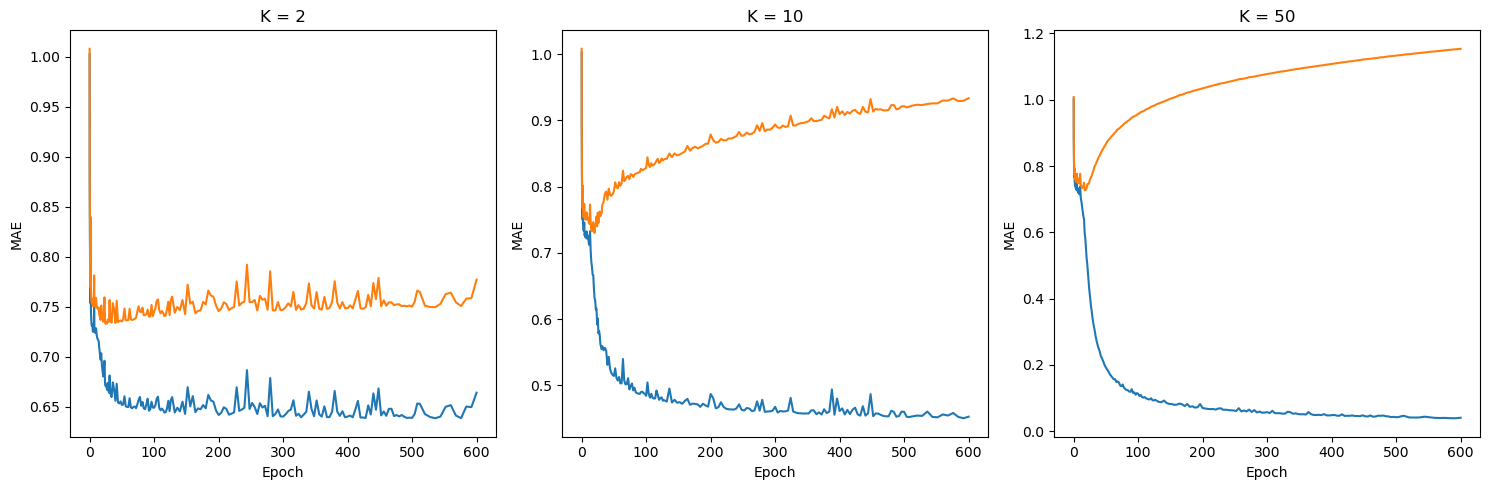
\includegraphics[width=\textwidth]{../images/Figure1a.png}
	\caption{All the graphs at first starts at a very high value of error. This is
  an indication of underfitting as the model has not yet been able to learned to
extract the pattern from the training data. As the number of epoch
increases, with SGD, we can see that the graphs of both training and validation
error began to converge. However, for all Ks, we can see that there is a sign of
overfitting as epochs go over 10. We can see that approximately at epoch 5, the
data began to converges and after 10, we can clearly see the separation between
training and validation error. Validation error went up while training error
went down significantly which indicates sign of overfitting of the model.}
\end{figure}
\subsection{Question 1b}
\subsubsection{Processes}
To select the best hyperparameters, we modified the SGD model for early stopping
and try out with different alphas, batch\_size and step\_size.

Below are the values that we've tried:
\begin{itemize}
  \item alphas: [0.0, 0.0001, 0.001, 0.1]
  \item batch\_sizes: [16, 32, 128, 1016]
  \item step\_sizes: [0.1, 0.3, 0.9, 2.7]
\end{itemize}

From 1a, we were able to see that most of the Ks values began to converges
around 200 epochs. Using this information, we began our search using epochs as
200. Using alpha as 0, we conduct hyperparameters search as seen below:

\noindent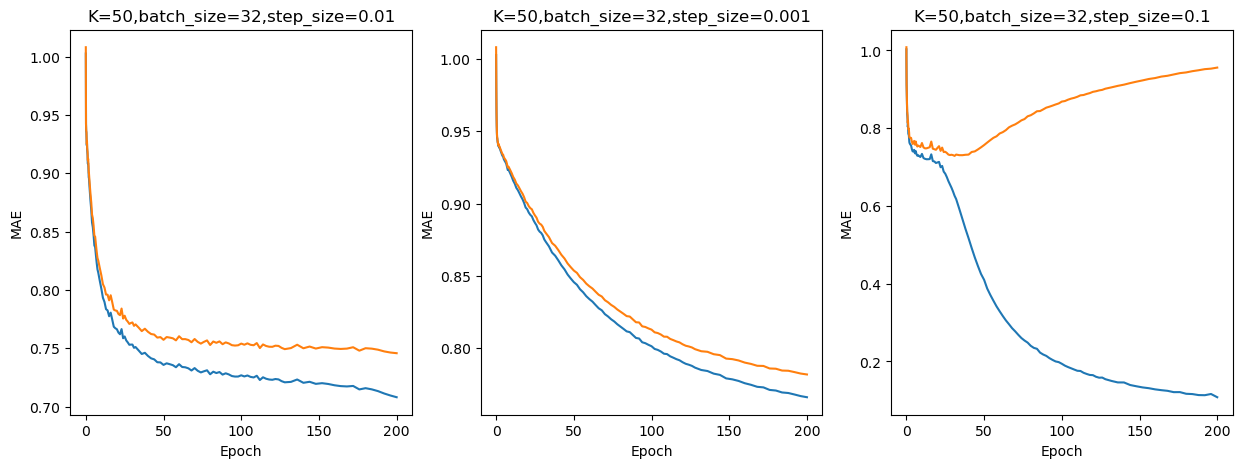
\includegraphics[width=\textwidth]{../images/1b-k50-bs32.png}

\noindent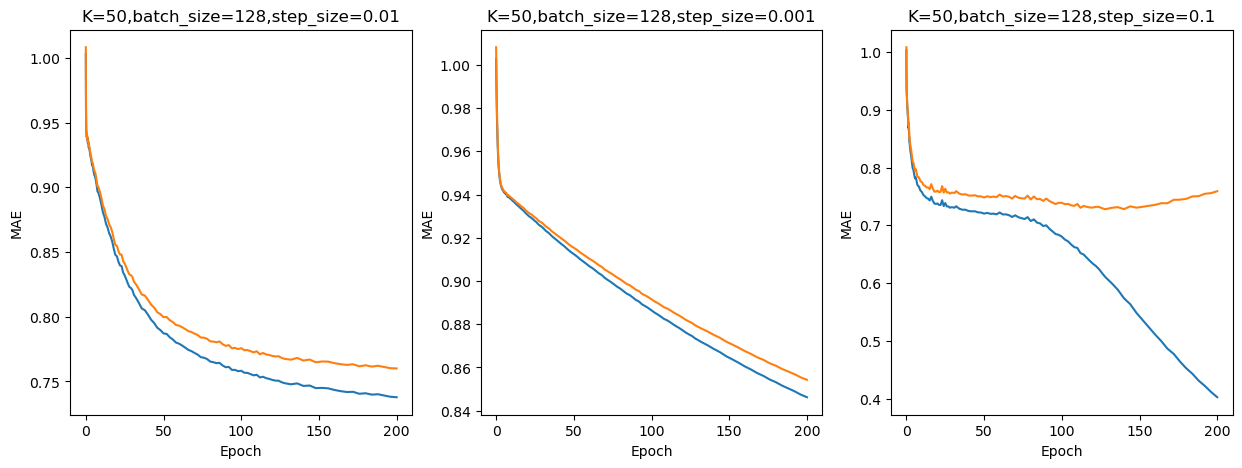
\includegraphics[width=\textwidth]{../images/1b-k50-bs128.png}

\noindent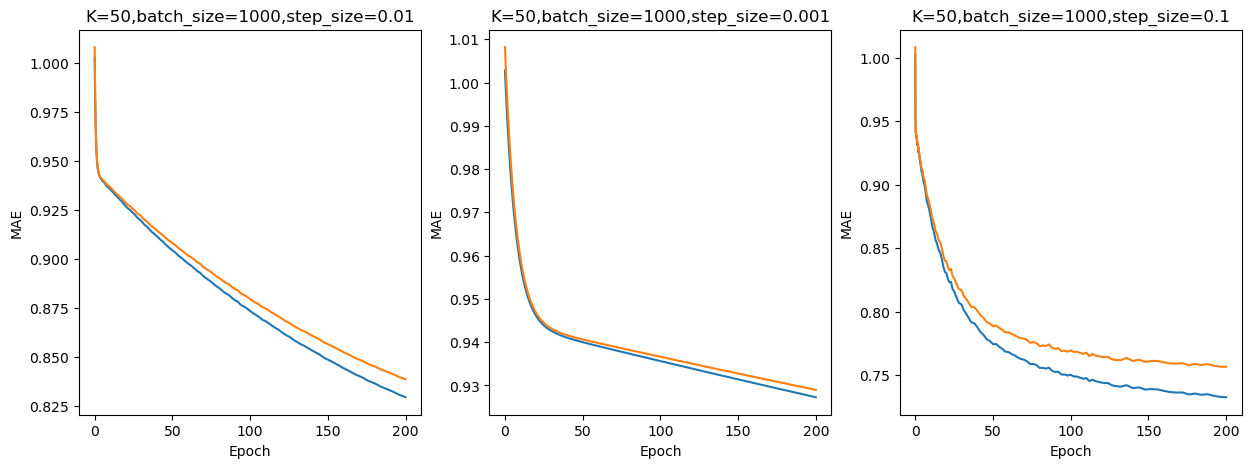
\includegraphics[width=\textwidth]{../images/1b-k50-bs1000.png}

With batch\_size of 1000 and step\_size of 0.1, we can see that it comes with
fast convergences in comparison to all other hyperparameters and able to achieve
the lowest training and validation errors. As for batch\_size of 32 and
step\_size 0.01, it's true that the combination provides fast convergences,
however, due to low batch\_size, the graph is not smooth + we can see signs of
overfitting when it's reaching 200 epochs.

\subsubsection{Figure 1b}
\begin{figure}[ht]
	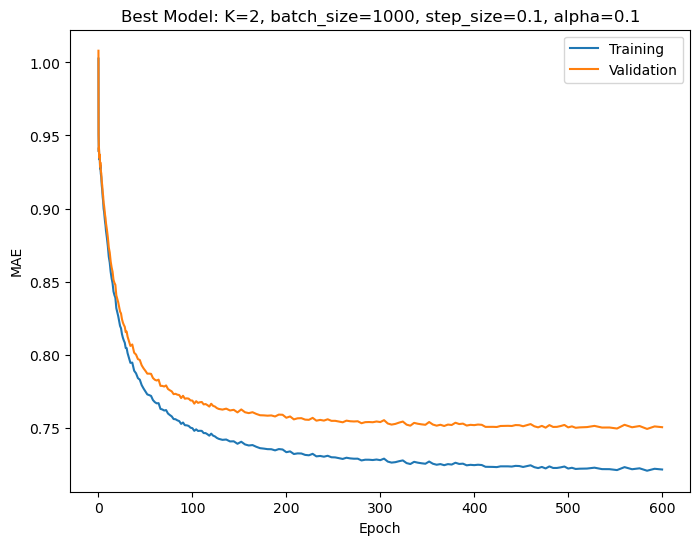
\includegraphics[width=\textwidth]{../images/Figure1b.png}
	\caption{For the best hyperparameters that achieved the best held out error,
  we were concluded that amongs the test values, alpha = 0.1, step\_size=0.1 and
batch\_size=1000 were able to achieves the lowest error on the heldout set. This
held out value was better than K=50 with 0.0 alpha as even though it wasn't able
to achieve low training errors as before, it was able to achieve an even higher
validation error.}
\end{figure}


\pagebreak
\subsection{Question 1c}
\begin{figure}[h]
	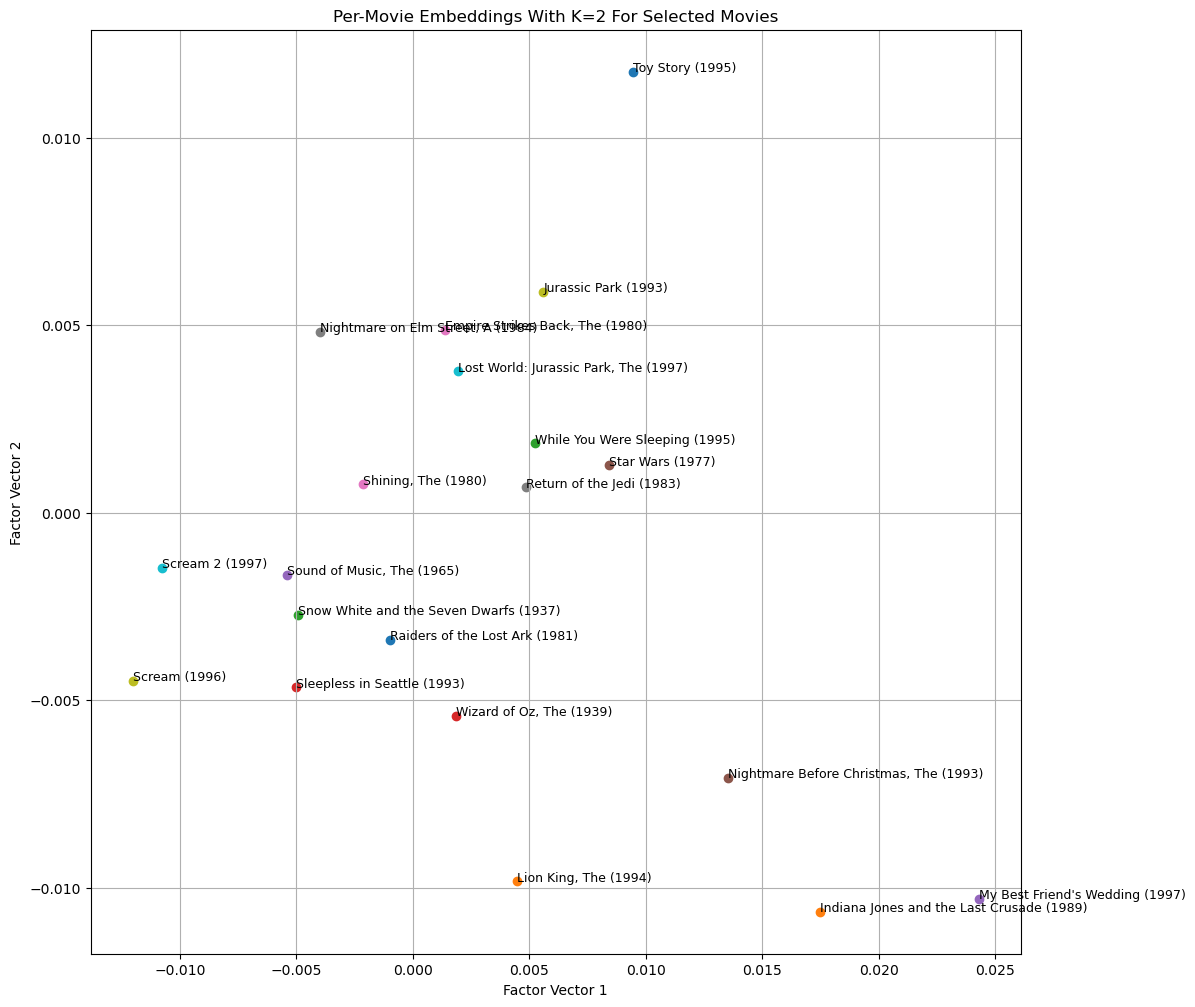
\includegraphics[width=\textwidth]{../images/Figure1c.png}
	\caption{
To select the best values for hyperparameters batch\_size, step\_size and alpha,
we began the hyperparameters search again with the ranges listed previously.
The best combination that achieves the lowest held-out error is
batch\_size=1000, step\_size=0.1, and alpha=0.1. Looking at the graph, we can
see that the movies that were categorized into the horror category like scream
is more on the negative side. Movies like Jurassic Park, Snow White and Star Wars are
extremely famous and popular are in nearer to the middle of the graph. While
movies like indiana jones, lion king, toy story and my best friend's wedding
which has a specific group of audience are more on the outer ring of the graph. This
indicates that as the vectors values more towards into the middle of the graph, the more
well received the movie is.}
\end{figure}


\section{Part 2}
\subsection{Question 2a}
For the features, besides the factor vector extracted using SVD algorithm, I
also used all the information in user\_info. For the item feature, I used only
the released date. For both of these, I obmitted the column orig\_user\_id and
orig\_item\_id as these two columns only matter if we are going to trace back
tot he 100k database for more information to extract from the movie. 

I was planning to perform TF-IDF extraction on the title of the movie. As we can
also get the importance of the words in the movie title as a feature for
classification as well. However, when append to the feature vector for training, the 
training time and memory requirement was increased exponentially as I train the
models and would not make it a good fit for the training.

\subsection{Question 2b}
For building the classifier, I chose GradientBoostingClassifier because it
provides the speed that I need for model selection. And for the second
classifier, I used Logistic Regression due to its simplicity and speed in
training. Initially, I was about to used kernelized SVM, however, the training took more
than 3 hours after I applied PCA and removed the TF-IDF vectorization of the
title. With that huge performance impact, I decided not to use it for this task.

For hyperparameters selection, I've performed grid search with the follow
settings:
\begin{enumerate}
  \item GradientBoostingClassifier:
    \begin{itemize}
      \item n\_estimator: [50,100,200]
      \item max\_depth: [3,5,7]
      \item learning\_rate: [0.01, 0.1, 0.2]
      \item subsample: [0.8,1.0]
    \end{itemize}
  \item LogisticRegression:
    \begin{itemize}
      \item C\: [0.01, 0.1, 1, 10, 100]
    \end{itemize}
\end{enumerate}

The best hyperparameters found are as below:
\begin{itemize}
  \item With K=2:
    \begin{enumerate}
      \item GradientBoostingClassifier:
        \begin{itemize}
          \item n\_estimator:200
          \item max\_depth:7
          \item learning\_rate:0.1
          \item subsample:0.8
        \end{itemize}
      \item LogisticRegression:
      \item C\:0.01
    \end{enumerate}
  \item With K=10:
    \begin{enumerate}
      \item GradientBoostingClassifier:
        \begin{itemize}
          \item n\_estimator:200
          \item max\_depth:5
          \item learning\_rate:0.2
          \item subsample:1.0
        \end{itemize}
      \item LogisticRegression:
      \item C\:0.01
    \end{enumerate}
  \item With K=50:
    \begin{enumerate}
      \item GradientBoostingClassifier:
        \begin{itemize}
          \item n\_estimator:200
          \item max\_depth:5
          \item learning\_rate:0.2
          \item subsample:0.8
        \end{itemize}
      \item LogisticRegression:
      \item C\:0.01
    \end{enumerate}
\end{itemize}
\subsection{Question 2c}
For each, I recorded the best AUC score during training evaluation on the
heldout set, not the AUC score against test set.

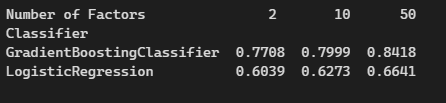
\includegraphics[width=\textwidth]{../images/Table 2c.png}
\end{document}


